% !TEX root = 7350.tex

\chapter{Berkovich spaces}

This generalizes Gelfand's theory. Much of the theory even works for 
non-commutative algebras. We do not require the existence of a base field, so 
our theory applies to ``arithmetic'' rings like $\bZ$ or 
$\bZ_2[x]/(7 x^3-5)$. 





\section{Berkovich spectrum of a normed ring}

We could phrase everything in terms of (rank-one) valuations and semivaluations.
Let $A$ be a commutative (unital) ring. 


\subsection{Norms and seminorms}

\begin{definition}
A \emph{seminorm} on $A$ is a function $\|\cdot\|\colon A\to \bR^{\geqslant 0}$ 
satisfying 
\begin{enumerate}
\item
$\|0\|=0$, $\|1\|\leqslant 1$, 

\item
$\|f+g\|\leqslant \|f\|+\|g\|$, 

\item
$\|f g\| \leqslant \|f\| \|g\|$. 
\end{enumerate}
\end{definition}

If we replace axiom 2 with $\|f+g\| \leqslant \max\{\|f\|,\|g\|\}$, we say the 
norm $\|\cdot\|$ is non-archimedean. We will focus primarily on non-archimedean 
norms. We allow $x\ne 0$ to have $\|x\|=0$. Define 
\[
  \ker(\|\cdot\|) = \{x\in A\colon \|x\| = 0\} .
\]
(Huber calls this the \emph{support} of $\|\cdot\|$.) This is a prime ideal in 
$A$. We call $\|\cdot\|$ a \emph{norm} if $\ker(\|\cdot\|)=0$. It turns out 
that our hypotheses imply that either $\|1\|=0$ or $\|1\|=1$. For, if 
$\|1\|\ne 0$, then $\|1\| \leqslant \|1\|\|1\|$, so $1\leqslant \|1\|$. If 
$\|1\|=0$, then $\|f\|=0$ for all $f\in A$. We want to allow this possibility 
so that the zero ring can have a norm. 

If $(A,\|\cdot\|)$ is a ring with seminorm, then $(A,+)$ is naturally a 
seminormed group, i.e.~it satisfies 
\begin{align*}
  \|0\| &=0 \\
  \|f+g\| &\leqslant \|f\|+\|g\| \\
  \|-f\| &= \|f\| .
\end{align*}
(Alternatively, replace the last two equations by 
$\|f-g\| \leqslant \|f\|+\|g\|$.) Any seminormed group carries a natural 
topology, so we get a topology on $A$. This topology is Hausdorff if and only 
if $\ker(\|\cdot\|)=0$. The (Hausdorff) completion $\widehat A$ exists (it can 
be defined via Cauchy sequences as usual), but the obvious map 
$Ai\colon\to \widehat A$ is injective if and only if $\ker(\|\cdot\|)=0$. In 
fact, $|ker(i)=\ker(\|\cdot\|)$. 

If we replace the axiom $\|f g\| \leqslant \|f\| \|g\|$ with 
$\|f g\| = \|f\| \|g\|$ and also assume $\|\cdot\|\ne 0$, we say that 
$\|\cdot\|$ is \emph{multiplicative}. If for all $f\in A$, $\|f^n\| = \|f\|^n$, 
we say $\|\cdot\|$ is \emph{power-multiplicative}. 

If $N$ is a subgroup of a seminormed group $(A,+)$, then we get a ``residue 
seminorm'' on $A/N$, defined by 
\[
  \|g+N\| = \inf\{\|f\|\colon f-g\in N\} .
\]
This gives a norm on $A/N$ if and only if $N$ is closed. 

Let $\varphi\colon M\to N$ be a homomorphism between seminormed groups. We call 
$\varphi$ \emph{bounded} if there exists some $C>0$ such that 
$\|\varphi(f)\|\leqslant C \|f\|$ for all $f\in M$. Clearly bounded functions 
are continuous. The converse does not hold in this level of generality. 

We say two seminorms $\|\cdot\|,\|\cdot\|'$ on a group are \emph{equivalent} if 
there exists $C_1,C_2>0$ such that 
\[
  C_1 \|\cdot\| \leqslant \|\cdot\|' \leqslant C_2 \|\cdot\| .
\]
Equivalent seminorms induce the same topology, but the converse is false in 
general. 

\begin{example}
Let $K$ be any field; consider $M=k[x]$. Let $f=\sum_0^n a_i x^i\in M$, and 
pick some $0<\alpha<1<\alpha'$. Define two seminorms on $M$ by:
\begin{align*}
  \|f\| &= \max\{\alpha^j\colon \alpha_j\ne 0\} \\
  \|f\|' &= \max\{{\alpha'}^j\colon \alpha_j\ne 0\} .
\end{align*}
Let $\varphi\colon (M,\|\cdot\|')\to (M,\|\cdot\|)$ be the identity on $M$. It 
is easy to check that $\varphi$ is bounded. Indeed, 
\[
  \frac{\|\varphi(f)\|}{\|f\|'} = \frac{\|f\|}{\|f\|'} = \frac{\alpha^j}{{\alpha'}^i} \leqslant 1 .
\]
Now $\varphi^{-1}$ is \emph{not} bounded (this is easy), but 
$\varphi^{-1}$ is continuous. We conclude that continuity does not imply 
boundedness. Moreover, bounded homeomorphisms need not have bounded inverses. 
\end{example}

Let $\varphi\colon M\to N$ be a linear map of seminormed groups. As groups, 
$M/\ker\varphi\simeq \image\varphi$, but this isomorphis might not respect the 
seminorms on the two groups. 

\begin{definition}
A linear map $\varphi\colon M\to N$ of seminormed groups is \emph{admissible} 
(or \emph{strict}) if the residue seminorm on $M/\ker\varphi$ and the seminorm 
on $\image\varphi$ are equivalent via the natural isomorphism 
$M/\ker\varphi\simeq \image\varphi$. 
\end{definition}

\begin{definition}
A \emph{Banach ring} is a normed ring which is complete (with respect to the 
norm). 
\end{definition}


\subsection{Examples and first properties}

\begin{example}
Any ring is with the trivial norm 
\[
  \|f\| = \begin{cases} 1 & \text{if }f\ne 0 \\ 0 & \text{if }f=0 \end{cases}
\]
is a Banach ring. 
\end{example}

\begin{example}
The ring $(\bZ,\|\cdot\|_\infty)$ is a Banach ring. The induced topology is 
discrete, but $\|\cdot\|_\infty$ is very far from being equivalent to the 
trivial norm on $\bZ$. 
\end{example}

\begin{example}
Let $A$ be a Banach ring, $\fa\subset A$ a closed ideal. Then $A/\fa$, with the 
residue norm, is a Banach ring. 
\end{example}

\begin{example}
In the context of the above example, if $\fm\subset A$ is any maximal ideal, 
then $A/\fm$ is a Banach field. Here we implicitly take advantage of 
\autoref{lem:maximal-ideal-closed}. 
\end{example}

\begin{lemma}\label{lem:maximal-ideal-closed}
Let $A$ be a Banach ring, $\fm\subset A$ a maximal ideal. Then $\fm$ is closed. 
\end{lemma}
\begin{proof}
If $\fa\subset A$ is any ideal, then its closure $\closure(\fa)$ is also an 
ideal. Of course, if $\fa$ is a proper ideal, then 
$\fa\cap A^\times=\varnothing$. But $A^\times$ is open. Indeed, if 
$x\in A^\times$, then $\disk^-(x,r)\subset A^\times$ for 
$r=\frac 1 2 \|x^{-1}\|^{-1}$. To see this, let $x+h\in \disk^-(x,r)$; we wish 
to show that $x+h\in A^\times$. We know that $\|h\|<\frac 1 2 \|x^{-1}\|^{-1}$, 
so $\|h x^{-1}\| \leqslant \|h\| \|x^{-1}\| < \frac 1 2$. Write 
$x+h=x(1+h x^{-1})$; the element $1+h x^{-1}$ is invertible by 
\autoref{lem:principle-units-invertible}
\end{proof}

\begin{lemma}\label{lem:principle-units-invertible}
Let $A$ be a Banach ring. Then $\disk^-(1,1)\subset A^\times$. 
\end{lemma}
\begin{proof}
We need to show that if $\|x\|<1$, then $1-x$ is invertible. The sequence 
\[
  a_n = 1 + x + \cdots + x^n ,
\]
is Cauchy because $\|x\|<1$, so it converges. One can easily check that the 
limit is $(1-x)^{-1}$. 
\end{proof}

\begin{example}\label{ex:Tate-algebra}
Let $A$ be a Banach ring with norm $\|\cdot\|$. Choose $r\in \bR^{>0}$. We 
define the ring $A\respow{r^{-1} T}\subset A\pow{T}$ to be the set of power 
series $f=\sum_{i\geqslant 0} a_i T^i$ such that 
$\sum \|a_i\| r^i< \infty$. If $A$ is non-archimedean, we only need to require 
$\|a_i\| r^i \to 0$. We call $A\respow{r^{-1} T}$ a ring of \emph{convergent 
power series}. We define a norm on $A\respow{r^{-1} T}$ by: 
\begin{align*}
  \|f\| &= \sum \|a_i\| r^i && \text{archimedean case} \\
  \|f\| &= \max\{ \|a_i\| r^i\} && \text{non-archimedean case} .
\end{align*}
We could have used the first definition in both cases, but the latter is easier 
to handle. Claim: $(A\respow{r^{-1} T},\|\cdot\|)$ is a Banach ring. 
\end{example}

\begin{example}
Let $\{A_i\}_{i\in I}$ be an arbitrary collection of Banach rings. Then the 
direct product $A=\prod A_i$ can be ``too large'' to be a Banach ring. It 
contains a natural Banach ring, namely the \emph{bounded direct product} 
\[
  \prod^\mathrm{b} A_i = \left\{(f_i)_{i\in I}\colon \sup\|f_i\|<\infty\right\} .
\]
This is a banach ring with respect to the norm 
$\|(f_i)\| = \sup \|f_i\|$. Also, there is the \emph{restricted direct 
product}:
\[
  \prod^\mathrm{c} A_i = \left\{(f_i)_{i\in I}\colon \lim \|f_i\|\to 0\right\} ,
\]
and the direct sum $\bigoplus_i A_i$. Note that the restricted direct product 
and direct sum will not be unital rings. 
\end{example}





\subsection{Spectrum: definition and first properties}

Let $(A,\|\cdot\|)$ be a normed ring. A seminorm $|\cdot|$ on $A$ is called 
\emph{bounded} (with respect to $\|\cdot\|$) if there exists $c>0$ such that 
$|f|\leqslant c\|f\|$ for all $f\in A$. One also calls bounded seminorms 
\emph{admissible}. If $|\cdot|$ is bounded, then the induced map 
$|\cdot|\colon A\to \bR,f\mapsto |f|$ is continuous, where $\bR$ has its usual 
topology and $A$ has the topology induced by $\|\cdot\|$. 

\begin{definition}
Let $A$ be a commutative unital Banach ring with fixed norm $\|\cdot\|$. The 
\emph{spectrum} of $A$, denoted $\Berkspec(A)$, is the set of bounded 
multiplicative seminorms on $A$. For $x\in \Berkspec(A)$, let $|\cdot|_x$ be 
the corresponding seminorm. We give $\Berkspec(A)$ the weakest topology making 
all maps $x\mapsto |f|_x$ continuous. 
\end{definition}

\begin{theorem}\label{thm:Berkspec-not-empty}
Let $A$ be a commutative Banach ring. Then 
\begin{enumerate}
\item
$\Berkspec(A)\ne\varnothing$. 

\item
$\Berkspec(A)$ is Hausdorff. 

\item
$\Berkspec(A)$ is compact. 
\end{enumerate}
\end{theorem}
\begin{proof}
1. This is the hardest part of the proof. Let $\fm\subset A$ be a maximal 
ideal; $\fm$ is closed by \autoref{lem:maximal-ideal-closed}. The quotient 
$A/\fm$ is a field, complete with respect to the residue norm. If 
$\Berkspec(A/\fm)\ne\varnothing$, then $\Berkspec(A)\ne\varnothing$. Indeed, 
if $|\cdot|$ is a bounded multiplicative seminorm on $A/\fm$, then 
$|\cdot|\colon A\to \bR$ given by $f\mapsto |f+\fm|$ is a bounded 
multiplicative seminorm on $A$. (This is a special case of functoriality: if 
$f\colon A\to B$ is a bounded homomorphism of Banach rings, there is a natural 
map $f^\ast\colon \Berkspec(B)\to \Berkspec(A)$.) Without loss of generality, 
we may assume that $A$ is a field. 

Let $S$ be the set of all non-zero bounded seminorms on $A$. Given 
$|\cdot|,|\cdot|'\in S$, we put $|\cdot|\leqslant |\cdot|'$ if 
$|f|\leqslant |f|'$ for all $f\in A$. This gives $S$ a partial order. Since 
$\|\cdot\|\in S$, the set $S$ is non-empty. If 
$\{|\cdot|_i\}_{i\in I}\subset S$ is a chain, then $\inf_i |\cdot|_i\in S$ is 
a lower bound for $\{|\cdot|_i\}_{i\in I}$. Zorn's lemma gives us a minimal 
element $|\cdot|\in S$. We claim that 
$|\cdot|$ is multiplicative. To show this, it's enough to show that 
$|f^{-1}| = |f|^{-1}$ for all $f\in A^\times$. For, we already know that 
$|f g|\leqslant |f| |g|$, so just compute:
\[
  |f g|^{-1} = |f^{-1} g^{-1}| \leqslant |f^{-1} |g^{-1}| = |f|^{-1} |g|^{-1} .
\]
We always have $1\leqslant |f| |f^{-1}|$, so assume there exists $f$ with 
$|f|^{-1}<|f^{-1}|$. Let $r=|f^{-1}|^{-1}<|f|$. Consider the 
Tate algebra (from \autoref{ex:Tate-algebra}):
\[
  B = A\respow{r^{-1} T} = \left\{\sum_{i\geqslant 0} a_i T^i\colon \sum |a_i| r^i < \infty\right\} .
\]
Note that $|\cdot|$ extends to $B$ by $|\sum a_i T^i| = \sum |a_i| r^i$. We 
claim that $f-T$ is not invertible in $B$. If it did have an inverse, this 
would be $\sum f^{-i} T^i$, which has norm $\sum |f^{-i}| r^i = \sum 1$, which 
diverges. (See the proof of \cite[1.2.1]{berkovich-1990} for details). Consider 
the map $A\to B/\langle f-T\rangle\ne\varnothing$. This induces a smaller 
bounded seminorm on $A$, which contradicts the minimality of $|\cdot|$. So 
$|\cdot|$ is multiplicative. 

2. For $x\ne y\in \Berkspec(A)$, we want to show there are disjoint open 
neighborhoods of $x$ and $y$. Since $x\ne y$, there exists some $f\in A$ such 
that $|f|_x\ne |f|_y$, say $|f|_x<|f|_y$. Choose $r\in \bR$ with 
$|f|_x<r<|f|_y$. Then $\{z\in \Berkspec(A)\colon |f|_z<r\}$ and 
$\{z\in \Berkspec(A)\colon |f|_z>r\}$ are the desired sets. 

3. Let $C=\prod_{f\in A} [0,\|f\|]$; this is compact by Tychonoff's theorem. 
Note that $\Berkspec(A)\hookrightarrow C$ via $x\mapsto (|f|_x)_{f\in A}$. 
Moreover, $\Berkspec(A)\subset C$ is closed because all the defining properties 
of $\Berkspec(A)$ are closed conditions. Thus $\Berkspec(A)$ is itself 
compact. 
\end{proof}

If $\|\cdot\|$ is already multiplicative, then $\Berkspec(A)\ne\varnothing$ 
because $\|\cdot\|\in \Berkspec(A)$. This is much harder in general. We didn't 
actually need the completeness of $A$ in the above definition. This is because 
any bounded seminorm on $A$ has a unique extension to $\widehat A$. We could 
have replaced $\|\cdot\|$ with any equivalent seminorm and get the same 
$\Berkspec(A)$. 

Let $|\cdot|\colon A\to \bR$ be a power-multiplicative bounded seminorm. Then 
$|f|^n \leqslant c\|f\|^n$; take $n$-th roots and let $n\to \infty$ to realize 
that we may assume $c=1$. So all $x\in \Berkspec(A)$ satisfy 
$|f|_x\leqslant \|f\|$ for all $f\in A$. 

The topology of $\Berkspec(A)$ is very mysterious. In general, one needs model 
theory to prove some basic facts (e.g.~that $\Berkspec(A)$ ``looks like'' a 
simplicial complex). Here are two equivalent ways to define the topology:
\begin{enumerate}
\item
The topology on $X=\Berkspec(A)$ is generated by open sets of the form 
\[
  \{x\in X\colon |f|_x<\alpha\} , \qquad \{x\in X\colon |f|_x>\alpha\} ,
\]
for $f\in A$, $\alpha\in \bR$. 

\item
A filter $\fF$ converges to $x\in X$ if and only if the filter 
\[
  |f|_\fF = \left\{\{|f|_u\colon u\in U\}\colon U\in \fF\right\} 
\]
converges to $|f|_x$ for all $f\in A$.  
\end{enumerate}

Let $x\in \Berkspec(A)$. Then $\fp_x = \ker(|\cdot|_x)$ is a closed prime 
ideal. For $f\in A$, $|f|_x$ depends only on $\bar f\in A/\fp_x$. But 
$|\cdot|_x$ is a bounded multiplicative norm on $A/\fp_x$. The ring $A/\fp_x$ 
is an integral domain, so we can pass to its field of fractions 
$(A/\fp_x)_{(0)}$, which carries the norm induced by $|\cdot|_x$. Let 
$\sH(x) = \widehat{(A/\fp_x)_{(0)}}$; this is the \emph{completed residue 
field} of $A$ at $x$. For $f\in A$, write $f(x)$ for the image of $f$ under the 
composite map 
\[
  A \twoheadrightarrow A/\fp_x \hookrightarrow (A/\fp_x)_{(0)} \hookrightarrow \widehat{(A/\fp_x)_{(0)}} = \sH(x) .
\]
We will write $|\cdot|$ for the canonical extension of $|\cdot|_x$ to 
$\sH(x)$. So $|f(x)| = |f(x)|_x = |f|_x$. The map $A\to \sH(x)$ is a 
``character,'' in the following sense. 

\begin{definition}
Let $A$ be a Banach ring. A \emph{character} on $A$ is a nonzero bounded 
homomorphism to a field complete with respect to some absolute value. 
\end{definition}

\begin{definition}
Let $A$ be a Banach ring. The \emph{Gelfand transform} on $A$ is the natural 
map 
\[
  A\to \prod^\mathrm{b}_{x\in \Berkspec(A)}  \sH(x) \qquad f\mapsto (f(x))_{x\in \Berkspec(A)} .
\]
\end{definition}

Let $B=\prod_{x\in \Berkspec(A)}^\mathrm{b} \sH(x)$. Then $B$ is a Banach ring, 
and the Gelfand transform $A\to B$ is a bounded map. We get an induced 
surjective map $\Berkspec(B)\to \Berkspec(A)$. 

\begin{lemma}
Let $A$ be a Banach ring. Then $f\in A$ is invertible if and only if 
$f(x)\ne 0$ for all $x\in \Berkspec(A)$. 
\end{lemma}
\begin{proof}
If $f\in A^\times$, then $|1|_x = |f f^{-1}|_x = 1$, so $|f|_x\ne 0$, whence 
$f(x)\ne 0$ in $\sH(x)$ for all $x$. If $f\notin A^\times$, then there is some 
maximal (hence prime) ideal $\fm\ni f$. By \autoref{thm:Berkspec-not-empty}, 
$\Berkspec(A/\fm)\ne\varnothing$. Choose $|\cdot|\in \Berkspec(A/\fm)$, and 
let $|\cdot|_x\in \Berkspec(A)$ be its pullback. Then 
$|f|_x = |f+\fm| = |\fm| = 0$. 
\end{proof}

Let $x\in \Berkspec(A)$. We have seen that there is a natural character 
$\chi_x\colon A\to \sH(x)$. Conversely, given a character $\chi\colon A\to K$, 
we get a bounded multiplicative seminorm $|\cdot|_\chi\colon A\to \bR$, defined 
by $|f|_\chi = |\chi(f)|$. At the moment, different characters might induce the 
same seminorm on $A$. We handle this by noting that two characters 
$\chi',\chi''$ give the same point in $\Berkspec(A)$ if and only if they are 
equivalent in the following sense: there exists a character $\chi\colon A\to K$ 
such that the following diagram commutes:
\begin{equation}\label{eq:equiv-characters}
\begin{tikzcd}
  & A \ar[dl, swap, "\chi'"] \ar[d, "\chi"] \ar[dr, "\chi''"] \\
  K' 
    & K \ar[l, hook] \ar[r, hook]
    & K''
\end{tikzcd}
\end{equation}


\subsection{Comparison with algebraic spectrum}

Let $A$ be a (commutative, unital) ring. Recall that $\spec(A)$ is the set of 
prime ideals in $A$, i.e.
\[
  \spec(A) = \{\fp\subset A\colon \fp\text{ is prime}\} .
\]
The set $\spec(A)$ has a topology with closed sets 
\[
  V_\fa = \{\fp\in \spec(A)\colon \fp\supset \fa\} ,
\]
where $\fa$ ranges over ideals in $A$. An \emph{algebraic character} on $A$ is 
a ring homomorphism from $A$ to a field, $\chi\colon A\to K$. 

Given $\fp\in \spec(A)$, we get a character 
\[
  \chi_\fp\colon A\twoheadrightarrow A/\fp \hookrightarrow (A/\fp)_{(0)} .
\]
Conversely, given a character $\chi\colon A\to K$, the ideal 
$\ker(\chi)\in \spec(A)$. Two characters $\chi',\chi''$ give the same point in 
$\spec(A)$ if and only if a diagram \eqref{eq:equiv-characters} exists in the 
algebraic category.

There is a natural map $\ker\colon \Berkspec(A)\to \spec(A)$ (the \emph{kernel 
map}), given by $|\cdot|\mapsto \ker(|\cdot|)$. This should not be mistaken for 
the specialization map we will encounter later. 

\begin{lemma}
\leavevmode
\begin{enumerate}
\item
The map $\ker\colon \Berkspec(A)\to \spec(A)$ is continuous. 

\item
If $\|\cdot\|$ (the fixed norm on $A$) is trivial, then 
\begin{enumerate}
\item
$\ker\colon \Berkspec(A)\to \spec(A)$ is surjective, 

\item
there is a canonical section $\spec(A)\to \Berkspec(A)$
\end{enumerate}
\end{enumerate}
\end{lemma}
\begin{proof}
1. Let $\fa\subset A$ be an ideal. We claim that  
\[
  \ker^{-1}(V_\fa) = \bigcap_{f\in \fa}\{x\in \Berkspec(A)\colon |f|_x = 0\} .
\]
Indeed, if $x$ lies in the right hand side, then for all $f\in \fa$, 
$|f|_x=0$, whence $f\in \fa\Rightarrow f\in \fp_x$, so we get 
$\fa\subset \fp_x$, i.e.~$\fp_x\in V_\fa$. This is equivalent to 
$\ker(|\cdot|_x)\subset V_\fa$, i.e.~$x\in \ker^{-1}(V_\fa)$. In fact, all the 
above implications are equivalences.

2. Givn $\fp\in \spec(A)$, define $|\cdot|_\fp\in \Berkspec(A)$ by 
\[
  |f|_\fp = \begin{cases} 0 & f\in \fp \\ 1 & f\notin \fp \end{cases} .
\]
Since $\|\cdot\|$ is trivial, $|\cdot|_\fp$ is a bounded multiplicative 
norm on $A$. The map $\fp\mapsto |\cdot|_\fp$ is the desired canonical 
section. 
\end{proof}


\subsection{Functoriality of \texorpdfstring{$\Berkspec$}{M}}

We want to show that $A\mapsto \Berkspec(A)$ is functorial in the appropriate 
sense. Let $\varphi\colon (A,\|\cdot\|)\to (B,\|\cdot\|')$ be a bounded 
homomorphism of commutative Banach rings. (As always, we assume that 
$\varphi(1)=1$.)

\begin{theorem}
\leavevmode
\begin{enumerate}
\item
The map $\varphi^\ast\colon \Berkspec(B)\to \Berkspec(A)$ given by 
$\varphi^\ast(|\cdot|') = |\cdot|$, $|f| = |\varphi(f)|'$, is well-defined and 
continuous. 

\item
Assume the set 
\[
  \left\{\frac{\varphi(f)}{\varphi(g)}\colon f,g\in A\text{ and }\varphi(g)\in B^\times\right\} 
\]
is dense in $B$. Then $\varphi^\ast$ is injective. 

\item
If $\varphi^\ast$ is injective, then $\Berkspec(B)$ is homeomorphic to its 
image in $\Berkspec(A)$. 
\end{enumerate}
\end{theorem}
\begin{proof}
1. That $|\cdot| = \varphi^\ast(|\cdot|')$ is multiplicative is obvious. To see 
that it is bounded, note that for all $f\in A$, we have 
\[
  |f| = |\varphi(f)|' \leqslant c_1 \|\varphi(f)\|' \leqslant c_1 c_2 \|f\| .
\]
Continuity follows from the fact that 
\[
  (\varphi^\ast)^{-1}\left(\{x\in \Berkspec(A)\colon |f(x)|>\alpha\}\right) = \{y\in \Berkspec(B)\colon |\varphi(f)(y)| > \alpha\} .
\]

2. Let $|\cdot|'\ne|\cdot|''\in \Berkspec(B)$ be such that 
$\varphi^\ast(|\cdot|') = \varphi^\ast(|\cdot|'')$. Then there exists $h\in B$ 
such that $|h|'\ne |h|''$, so we may as well assume $|h|'<|h|''$. Let 
$2\epsilon < |h|''-|h|'$. By assumption, there exists $f,g\in A$ such that 
$\varphi(g)\in B^\times$ and 
$\left\|h-\frac{\varphi(f)}{\varphi(g)}\right\|' < \epsilon$. Thus 
$\left|h-\frac{\varphi(f)}{\varphi(g)}\right| < \epsilon$ and 
$\left|h-\frac{\varphi(f)}{\varphi(g)}\right|'' < \epsilon$. Apply the triangle 
inequality:
\begin{align*}
  \left|\frac{\varphi(f)}{\varphi(g)}\right|' 
    &= \left|\frac{\varphi(f)}{\varphi(g)} - h+ h\right|' \\
    &\leqslant \left|\frac{\varphi(f)}{\varphi(g)} - h\right|' + |h|' \\
    &< \epsilon + |h|' \\
    &< |h|' - \epsilon .
\end{align*}
Similarly 
\begin{align*}
  |h|'' 
    &= \left|h - \frac{\varphi(f)}{\varphi(g)} + \frac{\varphi(f)}{\varphi(g)}\right|'' \\
    &\leqslant \left|h-\frac{\varphi(f)}{\varphi(g)}\right|'' + \left|\frac{\varphi(f)}{\varphi(g)}\right|'' \\
    &< \epsilon + \left|\frac{\varphi(f)}{\varphi(g)}\right|'' .
\end{align*}
It follows that 
$\left|\frac{\varphi(f)}{\varphi(g)}\right|' < \left|\frac{\varphi(f)}{\varphi(g)}\right|''$, 
so $|\varphi(f)|' |\varphi(g)|'' < |\varphi(f)|'' |\varphi(g)|'$. This implies 
$|f||g| < |f| |g|$, a contradiction. 

3. This follows from the general fact, proved in [Folland, p.129], that if 
$X$ is quasi-compact, $Y$ is Hausdorff, then any continuous bijection 
$f\colon X\to Y$ is a homeomorphism. 
\end{proof}

Note that the recurring norm 
\[
  |f|_\fp = \begin{cases} 1 & f\notin \fp \\ 0 & f\in \fp \end{cases} ,
\]
comes from the trivial seminorm on $A/\fp$. 



\subsection{Boundedness versus continuity for \texorpdfstring{$K$}{K}-algebras}

Usually (e.g., in classical algebraic geometry) one cares about rings that are 
also $K$-vector spaces, for some field $K$. 

\begin{definition}
Let $R$ be a commutative ring. A (unital, associative) \emph{$R$-algebra} is an 
abelian group $A$ equipped with the structure of both a (associative, unital) 
ring and an $R$-module, such that ring multiplication is $R$-bilinear in the 
sense that $r\cdot(x y) = (r\cdot x) y = x(r\cdot y)$. 
\end{definition}

It is equivalent to specify a (unital, associative) ring $A$ together with a 
ring homomorphism $R\to \zentrum(A)$, where 
$\zentrum(A)=\{a\in A\colon a b=ba\text{ for all }b\in A\}$ is the center of 
$A$. We are mainly interested in commutative $R$-algebras, but some aspects of 
the theory (especially over $\bC$) work just as well for possibly 
non-commutative algebras. 

Let $K$ be a field with absolute value, $A$ a $K$-algebra. A \emph{norm} 
$|\cdot|$ on $A$ is both a ring norm and a $K$-vector space norm. This in 
particular requires that $\|a v\| = |a| \| v\|$ for all $a\in K$, $v\in A$. 
So any norm on $A$ ``remembers'' the norm on $K$. More precisely, if $A$ is a 
normed $K$-algebra, $\|\cdot\|_x\colon A\to \bR$ a bounded multiplicative 
seminorm. Then $|\cdot|_x$ induces an absolute value on $\sH(x)$. But $\sH(x)$ 
is a complete extension of $K$. It turns out that $|\cdot|_x$ on $\sH(x)$ 
must restrict to $|\cdot|$ on $K$. This is Exercise 4.3.1 in Conrad's notes in 
\cite{aws-2008}.

Let $\varphi\colon A\to B$ be a $K$-algebra homomorphism. We assume that 
$A$ and $B$ have been given ($K$-)norms $\|\cdot\|$ and $\|\cdot\|'$. Clearly, 
if $\varphi$ is bounded (i.e.~$\|\varphi(f)\|' \leqslant c\|f\|$ for all 
$f\in A$), then $\varphi$ is continuous. We have seen that the converse does 
not always hold. 

Let's try working towards proving the converse. Let $\varphi\colon A\to B$ be a 
continuous homomorphism. Then $\varphi$ is continuous if and only if it is 
continuous at $0$. So there exists a neighborhood $U\ni 0$ such that 
$\varphi(U)\subset \{b\in B\colon \|b\|'<1\}$. There is $\delta>0$ such that 
$\{a\in A\colon \|a\|\leqslant \delta\}\subset U$. So 
$\|\varphi(x)\|'\leqslant 1$ whenever $\|x\|\leqslant \delta$. If we were 
working over $\bC$, we would not rescale. But this doesn't work if the norm on 
$K$ is trivial. If the norm $|\cdot|$ on $K$ is \emph{not} trivial (i.e., 
$|K^\times|\ne 1$) then by rescaling we can say that 
$\|x\|\leqslant |a|\Rightarrow \|\varphi(x)\|' \leqslant \frac{|a|}{\delta}$. 
So generally, $\|\varphi(x)\|' \leqslant \frac{1}{\delta}\|x\|$, and 
$\varphi$ is bounded. 

If $|\cdot|$ is trivial on $K$, then continuity does not imply boundedness. If 
$|\cdot|$ is nontrivial, many other (but not all) basic facts of functional 
analysis are also true, e.g.~Banach's open mapping theorem (a bijective bounded 
$K$-algebra homomorphism $A\to B$ has bounded inverse). 





\subsection{Gelfand's theory for \texorpdfstring{$K=\bC$}{K=C}}

Much of this material can be found in \cite[Ch.~10-11]{rudin-1991}. 
Here is our motivating example. 

\begin{example}
Let $X$ be a nonempty compact Hausdorff space. Let $A=\sC^0(X)$ be the space of 
continuous $\bC$-valued functions on $X$. With pointwise multiplication, $A$ is 
naturally a (commutative, unital) $\bC$-algebra. We give $A$ the supremum norm: 
\[
  \|f\| = \sup_{x\in X} |f(x)| .
\]
It's a standard fact that $A$ is complete, i.e.~it is a Banach $\bC$-algebra. 
\emph{Warning}: the norm on $\sC^0(X)$ is \emph{not} in general multiplicative, 
i.e.~we only have $\|fg\|\leqslant \|f\|\|g\|$.
\end{example}

\begin{example}
Let $X$ be a finite set with $n$ points. Then $C^0(X)=\bC^n$. 
\end{example}

It is natural to ask: ``given any commutative Banach $\bC$-algebra $A$, can we 
embed $A$ into $\sC^0(X)$ for some compact Hausdorff $X$?''

\begin{example}
We give $\Lp^1(\bR^n)$ the structure of a $\bC$-algebra via convolution:
\[
  (f\ast g)(x) = \int_{\bR^n} f(y) g(x-y)\, \mathrm{d} y .
\]
This makes $\Lp^1(\bR^n)$ a commutative, but non-unital algebra. We give 
$\Lp^1(\bR^n)$ a unit as follows. Let $A=\Lp^1(\bR^n)\oplus\bC\delta$, where 
$\delta$ is the ``Dirac delta'' with multiplication as follows:
\[
  (f_1+\lambda_1\delta) \ast (f_2+\lambda_2 \delta) = (f_1\ast f_2+\lambda_2 f_1 + \lambda_1 f_2) + \lambda_1 \lambda_2 \delta .
\]
Give $A$ a norm by 
\[
  \|f+\lambda\delta\| = \|f\|_{\Lp^1} + |\lambda| .
\]
\end{example}

\begin{example}
Let $X$ be a Banach space over $\bC$. Let $\sB(X)$ be the algebra of bounded 
linear operators on $X$, with $\|\cdot\|$ the operator norm. For example, if 
$\dim(X)=n$, then $\sB(X)\simeq M_n(\bC)$. Note that if $n>1$, then $\sB(X)$ is 
\emph{not} commutative. The theory of Gelfand-Mazur (and some of Berkovich's) 
work for non-commutative algebras as well. 
\end{example}

\begin{definition}
Let $A$ be a $\bC$-algebra. Put 
\[
  \sigma(f) = \{\lambda\in \bC\colon \lambda-f\notin A^\times\} .
\]
(In functional analysis, one calls $\sigma(f)$ the \emph{spectrum} of $f$, but 
we will avoid using this terminology. The complement 
$\bC\smallsetminus \sigma(f)$ is called the \emph{resolvent} of $f$.)
\end{definition}

For $K$ non-archimedean, one can give a definition for $\sigma(f)$, but it's 
quite a bit more complicated, so we won't reproduce it here. See 
\cite[Ch.~7]{berkovich-1990} for details. 

\begin{theorem}
Let $f\in A$. Then 
\begin{enumerate}
\item
$\sigma(f)\ne\varnothing$, 

\item
$\sigma(f)$ is compact. 
\end{enumerate}
\end{theorem}
\begin{proof}
Part 1 is essentially \autoref{lemma:spec-Banach}. For part 2, it suffices to 
show that $\sigma(f)$ is closed and bounded. That $\sigma(f)$ is closed follows 
(essentially) from the fact that $A^\times$ is open. For boundedness of 
$\sigma(f)$, see below. 
\end{proof}

\begin{definition}
For $f\in A$, put 
\[
  \rho(f) = \sup\{|\lambda|\colon \lambda\in \sigma(f)\} .
\]
\end{definition}

\begin{theorem}
$\rho(f) = \lim_{n\to \infty} \|f^n\|^{1/n}$. 
\end{theorem}
The proof will be given in a more general setting, after giving an equivalent 
definition of $\rho(f)$. 

\begin{definition}
Let $A$ be a Banach $\bC$-algebra. As a set, 
\[
  \cM(A) = \{\chi\colon A\to \bC\text{ a homomorphism of $\bC$-algebras}\} .
\]
\end{definition}

\begin{lemma}
\leavevmode
\begin{enumerate}
\item
Any $\chi\in \cM(A)$ is bounded.

\item
$\cM(A)$ can be identified with the space of maximal ideals in $A$ via 
$\chi\leftrightarrow \ker(\chi)$. 

\item
$\cM(A)=\Berkspec(A)$

\item
$f\in A^\times$ if and only if $\chi(f)\ne 0$ for all $\chi\in \cM(A)$. 

\item
$\lambda\in \sigma(f)$ if and only if $\chi(f)=\lambda$ for some 
$\chi\in \cM(A)$. 
\end{enumerate}
\end{lemma}
\begin{proof}
1. Use the fact that $\chi\colon A\to \bC$ respects the $\bC$-algebra structure 
of $A$. 

2. For $x\in \cM(A)$, $\sH(x)$ is a complete field containing $\bC$, we have 
$\sH(x)=\bC$. 

4. If $f\notin A^\times$, then $f\notin \fm$ for all $\fm$ maximal. 

5. Apply part 4 to $\lambda-f$. 
\end{proof}

Parts 2 and 3 essentially say that ``Berkovich analytification'' does 
\emph{not} produce any new points when we endow $\bC$ with the archimedean 
absolute value. When we endow $\bC$ with the trivial absolute value, the 
Berkovich analytification carries a lot of extra information. 

For $f\in A$, the \emph{Gelfand transform} of $f$ is the function 
$\hat f\colon \cM(A)\to \bC$ defined by 
\[
  \hat f(\chi) = \chi(f) .
\]
The Gelfand transform is \emph{a priori} a function $A\to \prod_{\cM(A)}\bC$. 
We have seen that $\rho(f) = \sup_{\chi\in \cM(A)} |\hat f(\chi)|$. Give 
$\cM(A)$ the weakest topology making each $\hat f$ continuous (this recovers 
the topology on $\Berkspec(A)$ we defined earlier). Then the Gelfand 
transform is a map $A\to \sC^0(\cM(A))$ and 
\[
  \rho(f) = \|\hat f\|_{\sC^0(\cM(A))} .
\]
Let $B=\{\hat f\colon f\in A\}\subset \sC^0(\cM(A))$. Clearly, the Gelfand 
transform gives us a $\bC$-algebra homomorphism 
$A\twoheadrightarrow B\hookrightarrow \sC^0(\cM(A)),f\mapsto \hat f$. What is 
the kernel of $A\twoheadrightarrow B$? Suppose $\hat f=0$, 
i.e.~$\hat f(\chi)=0$ for all $\chi$, i.e.~$\chi(f)=f\mod\ker(\chi)=0$ for all 
$\chi$. In other words, $\hat f=0$ if and only if $f\in \fm$ for all maximal 
ideals $\fm$ of $A$. So 
\[
  \ker(\hat\cdot) = \bigcap_{\fm\in \mathrm{mSpec}(A)} \fm = \text{Jacobson radical of } A  = \ker(\rho).
\]
So $\hat\cdot$ is injective if and only if $\rho$ is a norm (not just a 
seminorm) on $A$, if and only if $A$ is Jacobson semisimple. (We say a algebra 
$A$ is \emph{Jacobson semisimple} if its Jacobson radical vanishes.)

The algebra $A$ has a norm $\|\cdot\|$ already, while 
$B\subset \sC^0(\cM(A))$ carries the sup-norm. The map $\hat\cdot\colon A\to B$ 
is an sometry if and only if $\rho(\cdot)=\|\cdot\|$. Since $\rho$ is 
power-multiplicative, clearly a necessary condition is for $\|\cdot\|$ to be 
power-multiplicative. We will see later that $\rho(\cdot)=\|\cdot\|$ if and 
only if $\|\cdot\|$ is power-multiplicative. 

\begin{definition}[Old]
A $\bC$-Banach algebra $A$ is called \emph{uniform} if there exists a compact 
Hausdorff space $X$ such that there is a bounded $\bC$-algebra homomorphism
$A\hookrightarrow \sC^0(X)$ with image a closed subspace containing the 
constant functions and separating points of $X$. 
\end{definition}

(Recall that $S\subset \sC^0(X)$ \emph{separates points} if for any 
$x\ne y\in X$, there is $s\in S$ such that $s(x)\ne s(y)$.) An algebra 
$(A,\|\cdot\|)$ is uniform if and only if $\rho(\cdot)=\|\cdot\|$, if and only 
if $\|\cdot\|$ is power-multiplicative. 

Given a Banach $\bC$-algebra $(A,\|\cdot\|)$, one can always find a related 
uniform algebra $(A^\mathrm{u},\rho(\cdot))$. Namely, $A^\mathrm{u}$ is the 
completion of $A/\ker(\rho)$ with respect to the norm $\rho$. 

\begin{example}
Let $A=\Lp^1(\bR^n)\oplus \bC\delta$. Given any $\omega\in \bR^n$, we have a 
character $\chi_\omega\colon A\to \bC$, defined by 
\[
  \chi_\omega(f+\lambda\cdot\delta) = \hat f(\omega) + \lambda .
\]
Here, $\hat f$ is the usual Fourier transform of $f$. Also, there is the 
character 
\[
  \chi_\infty(f+\lambda\cdot \delta) = \lambda .
\]
It is known that 
$\cM(A) = \{\chi_\omega\}_{\omega\in \bR^n}\cup\{\chi_\infty\}$. So 
$\cM(A)$ is the ``spectrum'' space. Moreover, the (weak) topology on $\cM(A)$ 
is the same as the one-point compactification of $\bR^n$. 
\end{example}

As an exercise, make $[0,1]$ out of $[0,1]\cap \bQ$ by announcing what you 
would like to be your continuous functions on $[0,1]$. For a more formal 
discussion, see the introduction to \cite{berkovich-1990}. 

The theory of Gelfand-Mazur has another analytic generalization to 
C*-algebras and non-commutative geometry in the sense of A.~Connes. The 
``spectrum'' can be replaced by the \emph{unitary dual}, which plays a large 
role in the representation theory of real reductive groups. 





\subsection{Banach rings: the general case}

Let $A$ be a Banach ring, $f\in A$. 

\begin{definition}\label{def:general-spectral-radius}
The \emph{spectral radius} of $f$ is 
\[
  \rho(f) = \lim_{n\to \infty} \|f^n\|^{1/n} = \inf\{\|f^n\|^{1/n}\colon n\geqslant 1\} .
\]
\end{definition}

\begin{lemma}
\autoref{def:general-spectral-radius} makes sense. 
\end{lemma}
\begin{proof}
This follows from \autoref{thm:fekete} applied to $a_n=\log\|f^n\|$. The 
sequence is subadditive because $\|f^{n+m}\| \leqslant \|f^n\| \|f^m\|$.
\end{proof}

\begin{theorem}[Fekete]\label{thm:fekete}
Let $\{a_n\}_{n\geqslant 1}\subset \bR\cup\{-\infty\}$. If $\{a_n\}$ is 
subadditive ($a_{n+m}\leqslant a_n+a_m$), then 
$\lim_{n\to \infty} \frac{a_n}{n}$ exists and is equal to 
$\inf\{\frac{a_n}{n}\colon n\geqslant 1\}$. 
\end{theorem}
\begin{proof}
If $\inf\{\frac{a_n}{n}\colon n\geqslant 1\}=-\infty$, then it easily follows 
that $\lim \frac{a_n}{n}=-\infty$. 

Suppose the infimum is finite, and let 
$a=\inf\{\frac{a_n}{n}\colon n\geqslant 1\}$. Fix $\epsilon>0$, and let 
$k\gg 0$ be such that $\left|\frac{a_k}{k}-a\right|<\epsilon/2$. Let $l\gg 0$ 
be such that $\frac{a_r}{kl}<\epsilon/2$ for $r<k$. If $n>k l$, write  
$n=kq+r$ with $r<k$. Then $q\geqslant l$, so 
\[
  a \leqslant \frac{a_n}{n} \leqslant \frac{a_{kq}+a_r}{kq+r} \leqslant \frac{q a_k + kl\epsilon/2}{kq} = \frac{a_k}{k} + \frac{l\epsilon}{2q} < a+\epsilon .
\]
\end{proof}

Recall the Gelfand transform 
$\hat\cdot\colon A\twoheadrightarrow B\subset \prod^\mathrm{b}_{x\in \Berkspec(A)} \sH(x)$, given by 
\[
  \hat f(x) = f\mod{\ker|\cdot|_x} .
\]
The algebra $B$ inherits the supremum norm.  

\begin{theorem}[Spectral radius vs.~Berkovich spectrum]
Let $A$ be a commutative Banach ring. Then for all $f\in A$, 
$\rho(f) = \|\hat f\|$, i.e.~
\[
  \lim_{n\to \infty} \|f^n\|^{1/n} = \max_{x\in \Berkspec(A)} |f(x)| .
\]
\end{theorem}
\begin{proof}
First we show that 
$\lim_{n\to \infty} \|f^n\|^{1/n} \geqslant \max_{x\in \Berkspec(A)} |f(x)|$. 
Let $f\in A$ and $x\in\Berkspec(A)$. Then
\[
  \|f^n\| \geqslant |f^n|_x=|f|_x^n=|f(x)|^n,
\]
so $\rho(f)\geqslant |f(x)|$ and therefore $\rho(f)\geqslant \|\hat f\|$.

To show $\lim_{n\to \infty} \|f^n\|^{1/n} \leqslant \max_{x\in \Berkspec(A)} |f(x)|$, 
we will prove that for any $r\in \bR^{\geqslant 0}$, $\|\hat f \|<r$ implies 
$\rho(f)<r$. Fix $r$, and assume $\|\hat f\|<r$. Then, by boundedness, 
$|f(x)|<r$ for all $x\in\Berkspec(A)$. Let
\[
  A^\prime=\left\{ \sum_{i=0}^\infty a_iT^i : a_i\in A, \sum_{i=0}^\infty a_ir^{-i}<\infty \right\}
\]
be the ring of convergent power series with coefficients in $A$ having radius 
of convergence $r$. Note that $\sum_{i=0}^\infty a_ir^{-i}$ is a norm on 
$A^\prime$.

We claim that $1-fT$ is invertible in $A^\prime$. Assuming this claim, we have
\begin{align*}
  1-fT\text{ is invertible } 
    &\Leftrightarrow \sum_{i=0}^\infty f^iT^i\in A^\prime \\
    &\Leftrightarrow \sum_{i=0}^\infty a_ir^{-i}<\infty \\
    &\Rightarrow \| f^i \|r^{-i}<1 \text{ for }i\text{ sufficiently large} \\
    &\Rightarrow \|f^i\|^{\frac{1}{i}}<r \\
    &\Rightarrow \rho(f)<r,
\end{align*}
and we are done. To prove the claim, note that 
\begin{align*}
  1-fT\text{ is invertible in }A^\prime 
    &\Leftrightarrow (1-fT)(x)\neq 0 \;\forall x\in M(A^\prime) \\
    &\Leftrightarrow |1-fT|_x\neq 0 \;\forall x\in M(A^\prime)
\end{align*}
To show this it suffices to show $|fT|_x<1$ because
\[
  1=|1|_x=|1-fT+fT|_x\leqslant |1-fT|_x+|fT|_x
\]
and if $|1-fT|_x=0$ then the above inequality implies $1<0+1$.

To compute $|fT|_x$, note that $\|T\|=r^{-1}$. By assumption, we have $|f|_x<r$ 
for all $x\in \Berkspec(A)$. But the map
\[
  \Phi:A\to A^\prime
\]
sending $f\mapsto f$ induces an isometry
\[
  \Phi^\ast:\Berkspec(A^\prime)\to\Berkspec(A),
\]
so $|f|_x=|f|_{\Phi^*(x)}<r$ for all $x\in \Berkspec(A^\prime)$, and therefore
\[
|fT|_x=|f|_x|T|_x<rr^{-1}=1.
\]
\end{proof}
The following theorem shows that $\rho(\cdot)$ is a canonical seminorm
\begin{theorem}\label{thm:rho}
Let $(A,\|\cdot\|)$ be a commutative Banach algebra. Then
\begin{enumerate}
\item $\rho$ only depends on the equivalence class of $\|\cdot \|$.
\item $\rho:A\to\bR$ is a seminorm.
\item $\rho$ is always power-multiplicative.
\item $\rho(f)\leqslant\|f\|\;\forall f\in A$, moreover, $\rho(\cdot)=\|\cdot\|$ 
if and only if $\|\cdot\|$ is power-multiplicative.
\end{enumerate}
\end{theorem}
These results can be restated in terms of properties of the Gelfand transform
\begin{theorem}\label{thm:Gelfandtransform}
Let $\hat \cdot:A\to B$ be the Gelfand transform. Then
\begin{enumerate}
\item[(a)] $\ker \hat\cdot =\ker \rho$.
\item[(b)] $\hat\cdot$ is an isometry with respect to $(A,\|\cdot\|)$ and 
$(B,\rho(\cdot)$ if and only if $\|\cdot\|$ is power-multiplicative.
\end{enumerate}
\end{theorem}
The ideal $\ker\rho$ is called the \emph{quasinilradical} of $A$. Its elements 
are the quasinilpotents of $A$, i.e.~those elements $f$ of $A$ for which
\[
  f(x)=0 \;\forall x\in \Berkspec(A).
\]
In algebraic geometry, $f\in R$ is identically zero on $\spec(R)$ if and only 
if
\[
  f(\fp)=f+\fp=0\quad \forall\fp\in\spec(R).
\]
which happens if and only if
\[
  f\in\bigcap_{\fp\in\spec(R)}\fp=\text{rad}(\langle 0\rangle),
\]
which is known as the nilradical of $R$.

Note that the nilradical is contained in the quasinilradical because of the 
power-multiplicativity of $\rho$. Recall that we have shown that for 
$\bC$-Banach algebras, the quasinilradical is equal to the Jacobson radical of 
$A$.

\begin{definition}\label{def:uniform}
A Banach algebra $(A,\|\cdot\|)$ is called \emph{uniform} if $\|\cdot\|$ is 
power-multiplicative.
\end{definition}
\begin{lemma}\label{lem:squaresonly}
$\|\cdot \|$ is power-multiplicative if and only if for all $f\in A$, 
$\| f^2\|=\|f\|^2$.
\end{lemma}
\begin{proof}
Fix $f$. Define $\Phi(n)=\log \|f^n\|$. By assumption, we have
\[
  \Phi(2)=2\Phi(1)
\]
so $\Phi(2^m)=2^m\Phi(1)$. We want $\Phi(n)=n\Phi(1)$. Note: $\Phi$ is 
subadditive, so $\Phi(n)\leqslant n\Phi(1)$. If $\Phi(n)<n\Phi(1)$, then let 
$k$ be such that $k+n=2^m$. Then
\[
  2^m\Phi(1)=\Phi(2^m)=\Phi(k+n)\leqslant \Phi(k)+\Phi(n)<k\Phi(1)+n\Phi(1)=2^m\Phi(1)
\]
which is a contradiction.
\end{proof}

\begin{proof}[Proof of \autoref{thm:rho}]
Let 
\begin{align}\label{eq:def1}
  \rho(f) &= \lim_{n\to \infty} \|f^n\|^{1/n}) \\ \label{eq:def2}
  \rho(f) &= \max_{x\in \Berkspec(A)} |f(x)|
\end{align}
denote the two equivalent definitions of $\rho$. 
\begin{enumerate}
\item
This follows immediately from \eqref{eq:def1}.

\item
$\rho(0)=0,\rho(1)=1$ and $\rho(fg)\leqslant\rho(f)\rho(g)$ follow from 
\eqref{eq:def1}, $\rho(f+g)\leqslant\rho(f)+\rho(g)$ follows easily from 
\eqref{eq:def2}.

\item
\eqref{eq:def1}

\item
By \eqref{eq:def1}, we have 
$\rho(f)=\lim_{n\to\infty} \|f^n\|^{\frac{1}{n}}\leq \lim_{n\to\infty}\|f\|^{n\frac{1}{n}}=\|f\|$. 
If $\rho=\|\cdot\|$, then by 3, $\|\cdot\|$ is power-multiplicative, so 
$\rho(f)=\|f^n\|^{\frac{1}{n}}=\|f\|$.
\end{enumerate}
\end{proof}
\begin{proof}[Proof of \autoref{thm:Gelfandtransform}]
\begin{enumerate}
\item[(a)] Follows from \eqref{eq:def1}.
\item[(b)] Follows from \autoref{thm:rho}, 4.
\end{enumerate}
\end{proof}
Recall that the kernel map $\ker\colon\Berkspec(A)\to\spec(A)$ sending 
$x\mapsto \ker |\cdot|_x$ is continuous with respect to the Berkovich topology 
on $\Berkspec(A)$ and the Zariski topology on $\spec(A)$.

\begin{definition}\label{def:zariskiberkspec}
The Zariski topology on $\Berkspec(A)$ is the weakest topology making $\ker$ 
continuous.
\end{definition}

As an exercise, show that $\Berkspec(A)$ is irreducible with respect to the 
Zariski topology if and only if $\ker\rho$ is a prime ideal.


\subsection{Uniformization of Banach Rings}

Let $(A,\|\cdot\|)$ be a Banach Ring. We would like to find a uniform 
Banach Ring associated to $A$. Motivated by \autoref{thm:rho}, we would like to 
use $\rho$, but as seen in that theorem, $\rho$ is in general only a seminorm, 
and $A/\ker\rho$ might not be complete. Therefore we define the uniformization 
$A^\mathrm{u}$ of $A$ to be
\[
  A^\mathrm{u}=\widehat{A/\ker \rho}
\]
where $\hat{\cdot}$ refers to completion with respect to $\rho$. Then 
$(A^\mathrm{u},\rho)$ is a uniform Banach ring (we denote the residue norm of 
$\rho$ by $\rho$ again). Let $\pi\colon A\to A^\mathrm{u}$ be the quotient map.

\begin{theorem}\label{thm:uniformization}
\leavevmode
\begin{enumerate}
\item For any bounded morphism $\phi\colon A\to B$ with $B$ uniform we have
\[
\begin{tikzcd}
  A \ar[dr, "\phi"] \ar[r, "\pi"]
    & A^\mathrm{u} \ar[d, dotted, "\exists !"] \\
  & B
\end{tikzcd}
\]
\item We have $\Berkspec(A^\mathrm{u}) = \Berkspec(A)$.
\item $\Berkspec(A^\mathrm{u})$ has one point if and only if $A^\mathrm{u}$ is 
a field and $\rho$ is an absolute value on $A^\mathrm{u}$.
\item $\rho$ is non-archimedean on $A^\mathrm{u}$ if and only if for all 
$x\in \Berkspec(A^u)$, $(\sH(x),{|\cdot|_x})$ is non-archimedean.
\end{enumerate}
\end{theorem}
\begin{proof}
1. By a similar trick as before, using power-multiplicativity of $\|\cdot\|_B$, we may assume
\[
  \|\phi(f)\|_B\leqslant \rho(f).
\]
So if $\rho(f)=0$ then $\phi(f)=0$ and $\phi\colon A\to B$ factors through 
$\pi\colon A\to A^\mathrm{u}$.

2. The map $\pi\colon A\to A^\mathrm{u}$ is bounded since it's a quotient map. Then
\[
  \pi^\ast\colon \Berkspec(A^\mathrm{u})\to\Berkspec(A)
\]
is injective, since $\pi(A)$ is dense in $A^\mathrm{u}$. Both $\Berkspec(A^\mathrm{u})$ 
and $\Berkspec(A)$ are compact Hausdorff spaces, so injectivity of $\pi$ implies
\[
  \Berkspec(A^\mathrm{u})\simeq \pi\left( \Berkspec(A^\mathrm{u}) \right),
\]
so we just need to show that $\pi^\ast$ is surjective. Let 
$|\cdot|_x\in \Berkspec(A)$. Note that it suffices to give such a 
$|\cdot|_y\in\Berkspec(A/\ker\rho)$, since then $|\cdot|_y$ will extend uniquely 
to the completion $A^\mathrm{u}$. Define
\[
  |f+\ker\rho|_y=|f|_x=|f(x)|.
\]
This is well-defined as $\rho(f)=\max_{x\in\Berkspec(A)}|f(x)|=0$ implies $f(x)=0$ 
for all $x$.

3. $\Leftarrow$. If $(K,|\cdot|)$ is a field with absolute value, then 
$\Berkspec(K)$ is a point, because for any $x\in \Berkspec(K)$, 
$\ker|\cdot|=0$. Thus $\sH(x)=K$, and the character $K\to \sH(K)$ is the 
identity. 

$\Rightarrow$. Suppose $\Berkspec(A^\mathrm{u}) = \{x\}$. First, we claim that 
$\rho(\cdot)$ is multiplicative, which follows from \eqref{eq:def2}. Next, we 
know that $f\in (A^\mathrm{u})^\times$ if and only if $f(x)\ne 0$. Thus 
$x=\rho$, so $(A^\mathrm{u})^\times = A\smallsetminus \ker\rho = 0$. We have 
shown that $A^\mathrm{u}$ is a field. 

4. Assume that for all $x\in\Berkspec(A^\mathrm{u})$, $(\sH(x),|\cdot|_x)$ is 
non-archimedean. Then as
\[
  \rho(f)=\max_{x\in\Berkspec(A^\mathrm{u})}|f(x)|=\max_{x\in\Berkspec(A^\mathrm{u})}|f|_x,
\]
$\rho$ is non-archimedean.

For the converse, recall that it suffices to check the archimedean property for 
integers. Assume that $\rho$ is non-archimedean. Then $\rho(n)\leqslant 1$ for all 
$n\in\bZ$. Therefore for $x\in\Berkspec(A^\mathrm{u})$,
\[
  |n|_x\leqslant\rho(n)\leqslant 1 ,
\]
so $|\cdot|_x$ is non-archimedean.
\end{proof}



\subsection{Products}

Let $(A,\|\cdot\|_A)$ be a normed ring.
\begin{definition}\label{def:modules}
A \emph{seminorm} on an  $A$-module $M$ is a function
\[
  \|\cdot\|:M\to\bR
\]
such that
\begin{enumerate}
\item
\begin{itemize}
\item $\|0\|=0,$
\item $\|m+n\|\leqslant \|m\|+\|n\|,$
\item $\|m\|=\|-m\|.$
\end{itemize}
\item There exists some $c>0$ such that for all $f\in A,m\in M$,
\[
\|f\cdot\|\leqslant c\|f\|_A\|m\|.
\]
\end{enumerate}
\end{definition}
\emph{Fact:} We may assume $c=1$ by replacing $\|\cdot\|$ by $\|\cdot\|^\prime$, defined as
\[
\|m\|^\prime=\sup_{f\in A\setminus\{0\}}\frac{\|f\cdot m\|}{\|f\|_A}.
\]
Then
\[
\|m\|\leqslant \|m\|^\prime\leqslant c\|m\|
\]
so $\|\cdot\|$ is equivalent to $\|\cdot\|^\prime$.

Let $M$ and $N$ be $A$-modules. On the tensor product $M\otimes_A N$ we have some natural choices for seminorms.
\begin{enumerate}
\item If $A,M,N$ are all archimedean, then for $s\in M\otimes_A N$, let
\begin{align}
\|s\|&=\inf \left( \sum_{i\in I}\|m_i\|\|n_i\| \right),\label{def:archtensor}
\end{align}
where we are taking the infimum of the above for all presentations of $s$:
\begin{align}
s&=\sum_{i\in I} m_i\otimes n_i.\label{def:nonarchtensor}
\end{align}
\item If $A,M,N$ are all non-archimedean, we prefer the following choice
\[
\|s\|=\inf \left( \text{Max}_{i\in I} \|m_i\|\|n_i\| \right)
\]
\end{enumerate}
Some remarks about this definition:
\begin{enumerate}
\item Definition \eqref{def:archtensor} also makes sense in the non-archimedean setting, but the two definitons are nonequivalent in general.
\item Definition \eqref{def:nonarchtensor} will not work in the archimedean case.
\item Even when the seminorms on $M$ and $N$ are norms, the seminorm on $M\otimes_A N$ might have a nontrivial kernel.
\item In general $M\otimes_A N$ is not complete.
\end{enumerate}
To remedy this, we define
\[
  M\hat{\otimes}_AN=\widehat{M\otimes_A N}
\]
where completion is taken with respect to the above-defined norm. Then $M\hat{\otimes}_AN$ is also an $\hat{A}$-module.

Note that the map
\[
M\otimes_A N\to M\hat{\otimes}_AN
\]
is not in general injective.
\begin{theorem}[Gruson] Let $K$ be a non-archimedean complete field, $M$ and $N$ be $K$-Banach vector spaces. Then the natural map 
\[
  M\otimes_A N\to M\hat{\otimes}_AN
\]
is injective.
\end{theorem}
The completed tensor product $M\hat{\otimes}_AN$ also has the following universal property: Any bounded bilinear map $M\times N\to L$ where $L$ is a complete normed $A$-module factors through the canonical map
\[
M\times N\to M\hat{\otimes}_A N.
\]
Our main interest in tensor products is extension of scalars, i.e. if $A$ is a $K$-Banach algebra and $L/K$ is a field extension, we want to study
\[
A^\prime=A\hat{\otimes}_K L
\]





\section{Behavior of \texorpdfstring{$\Berkspec(A)$}{M(A)} with respect to field extension}

One motivation is: let $A$ be a $\bQ_p$-algebra. We would like to understand 
$X_{\bQ_p}=\Berkspec(A)$ in terms of 
$X_{\bC_p} = \Berkspec(A\hat\otimes_{\bQ_p}\bC_p)$. Another reason is that by 
extending the base field, we can enlarge the value group. For example, we can 
obtain value group $\bR$, which makes some things easier. 

Let $A,B$ be Banach $K$-algebras, and put $X=\Berkspec(A)$, $Y=\Berkspec(B)$. 
We have a commutative diagram 
\[
\begin{tikzcd}
	K \ar[r] \ar[d]
		& A \ar[d] \\
	B \ar[r]
		& A\hat\otimes_K B ,
\end{tikzcd}
\]
which (by functoriality) gives us a commutative diagram of spectra:
\[
\begin{tikzcd}
	\Berkspec(A\hat\otimes_K B) \ar[r] \ar[d]
		& X \ar[d] \\
	Y \ar[r]
		& \{\ast\} .
\end{tikzcd}
\]
We put $X\times_K Y = \Berkspec(A\hat\otimes_K B)$. There are projection maps 
$X\times_K Y\to X$ and $\to Y$, corresponding e.g.~to the maps 
$A\to A\hat\otimes_K B$, $f\mapsto f\otimes 1$. Write 
$\pi\colon X\times_K Y\to X$. Given $x\in X$, what is the fiber $\pi^{-1}(x)$? 
It turns out that $\pi^{-1}(x)\simeq\Berkspec(\sH(x)\hat\otimes_K B)$. That is, 
topological and ``algebraic'' fibers agree. So in particular, 
$\pi^{-1}(x)\ne\varnothing$ for all $x$, so $X\times Y\to X$ is surjective. The 
algebraic incarnation of $\pi^{-1}(x)\hookrightarrow X\times Y$ is the map 
$A\hat\otimes_K B\to \sH(x)\otimes_K B$. Since $\pi^{-1}(x)$ is compact 
Hausdorff, the injection $\psi^\ast\colon\pi^{-1}(x)\hookrightarrow X\times Y$ 
is a homeomorphism onto its image. 


\subsection{Fibers in algebraic geometry}

See [Hartshorne]. Let $f\colon X\to Y$ be a morphism of schemes, 
$y\in Y=\spec(R)$. The fiber over $y$, written $f^{-1}(y)$, is defined to be 
the fiber product $X\times_Y \spec(k(y)) = X\times_Y y$. 





\subsection{Rigid geometry}

Let $K$ be a non-archimedean field, $L/K$ a field extension, and $A$ a Banach 
$K$-algebra. Write $X=\Berkspec(A)$ and $X_L=\Berkspec(A\hat\otimes_K L)$. From 
the above discussion, we have a surjective continuous map $X_L\to X$. 




\subsection{Interlude in Galois theory}

Let $K$ be a field; fix an algebraic closure $\overline K$. Let $L/K$ be an 
algebraic (but possibly infinite) extension. We say that $L/K$ is:
\begin{itemize}
\item
\emph{normal} if all $K$-embeddings $L\hookrightarrow \overline K$ have the 
same image. Let $\aut(L/K)$ be the group of field automorphisms of $L$ which 
are trivial on $K$. For example, $\bQ(\sqrt[3]{2})/\bQ$ is not normal, but 
$\bQ(\sqrt[3]{2},\zeta_3)/\bQ$ is normal. 

\item
\emph{separable} if for all $\alpha\in L$, the minimal polynomial 
$f\in K[x]$ of $\alpha$ has distinct roots in $\overline K$. Equivalently, 
$L\otimes_K \overline K$ is reduced. Any field extension in characteristic 
zero is separable, as are all extensions of finite fields. More generally, any 
extension of a perfect field is separable. (A field $K$ is \emph{perfect} if 
either $K$ is characteristic zero or all $x\in K$ are of the form $y^p$ for 
some $y\in K$.) For $p$ a prime, the extension $\bF_p(\sqrt[p]{t})/\bF_p(t)$ is 
not separable. 

\item
\emph{purely inseparable} if for any $\alpha\in L\smallsetminus K$, the minimal 
polynomial of $\alpha$ has repeated roots. Equivalently, if $K$ has 
characteristic $p>0$, the extension $L/K$ is purely inseparable if and only if 
for any $\alpha\in L$, there exists $n\geqslant 0$ such that 
$\alpha^{p^n}\in K$. 

\item
\emph{Galois} if it is normal and separable. Alternatively, 
$\# \aut(L/K)=[L\colon K]$, or $L^{\aut(L/K)} = K$. 
\end{itemize}

Artin proved a ``primitive element theorem'' for Galois extensions. One 
corollary is that if $L/K$ is finite separable, then $L=K(\alpha)$ for some 
$\alpha\in L$. Any algebraic extension $L/K$ has a distinguished 
subset 
\[
	S = \{\alpha\in L\colon \text{the minimal polynomial of $\alpha$ is separable}\} .
\]
One can check that $S$ is a field. Moreover, $S/K$ is separable, and $L/S$ is 
purely inseparable. 

Let $L/K$ be an algebraic Galois extension with Galois group $G=\galois(L/K)$. 
Let $\fF=\{K\subset K'\subset L\colon K'/K\text{ finite Galois}\}$. The group 
$G$ naturally carries a topology (the \emph{Krull topology}); a basis of 
neighborhoods of $1\in G$ is given by 
\[
  \{\galois(L/K')\colon K'\in \fF\} .
\]
Moreover, 
\[
  \galois(L/K) = \varprojlim_\fF \galois(K'/K) ,
\]
as topological groups, where we give each $\galois(K'/K)$ the discrete 
topology. So $\galois(L/K)$ is a profinite group. Given any tower 
$K_2/K_1/K$ of Galois extensions, we have a short exact sequence of profinite 
groups:
\[
  1 \to \galois(K_2/K_1) \to \galois(K_2/K) \to \galois(K_1/K)\to 1 .
\]

If $L/K$ is an algebraic extension that is not normal, the \emph{normal 
closure} of $L$ (over $K$) is the composite of all images of $K$-embeddings 
$L\hookrightarrow \overline K$. If we write $L'$ for the normal closure of 
$L$, then $L'/L$ is normal, and $L'$ is the smallest normal extension of $L$ 
which contains $L$. If $[L\colon K]<\infty$, then $[L'\colon K]<\infty$. 

\begin{lemma}
If $L/K$ is normal and purely inseparable, then $\aut(L/K)=1$. 
\end{lemma}
\begin{proof}
Actually, purely inseparable extensions are automatically normal. We need to 
show that for all $\sigma\in \aut(L/K)$ and $a\in L$, we have $\sigma(a)=a$. 
Assume $L$ has characteristic $p>0$. Given $a\in L$, there exists 
$n\geqslant 0$ such that $a^{p^n}\in K$. Then 
$\sigma(a)^{p^n} = \sigma(a^{p^n}) = a^{p^n}$. Thus 
$(\sigma(a)-a)^{p^n}=0$, so $\sigma(a)=a$. 
\end{proof}



\subsection{Completion of normal extensions}

Let $L/K$ be an (algebraic) normal extension. Suppose we have an absolute 
value $|\cdot|$ on $K$, for which $K$ is complete. We have seen that there is a 
unique extenion of $|\cdot|$ to $L$. If $[L\colon K]<\infty$, then $(L,|\cdot|)$ 
is complete. If not, let $\widehat L$ denote its completion. 

\begin{lemma}
The extension $\widehat L/K$ is normal, and $L\hookrightarrow \widehat L$ 
induces an isomorphism $\aut(\widehat L/K)\xrightarrow\sim \aut(L/K)$. 
\end{lemma}
\begin{proof}
The archimedean case can be checked directly, so we suppose $K$ (and hence $L$) 
is non-archimedean. Note that any $\sigma\in \aut(L/K)$ is an isometry with 
respect to $|\cdot|$. This follows from the norm-formula:
\[
  |x| = \left|\norm_{K(x)/K}(x)\right|^{[K(x)\colon K]^{-1}} ,
\]
which is clearly $\aut(L/K)$-invariant. Alternatively, use the fact that for 
any $\sigma\in \aut(L/K)$, the pullback $\sigma^\ast |\cdot|$ is also an 
extension of $|\cdot|$ to $L$, so uniqueness tells us that 
$\sigma^\ast|\cdot|=|\cdot|$, i.e.~$|\cdot|$ is $\sigma$-invariant. Thus any 
$\sigma\in \aut(L/K)$ extends by continuity to an element of 
$\aut(\widehat L/K)$. 
\end{proof}



\subsection{Action of \texorpdfstring{$\aut(\widehat L/K)$}{Aut(L/K)} on Berkovich spectra}

Let $L/K$ be a normal extension of complete non-archimedean fields. Let 
$A$ be a Banach $K$-algebra. Write $A_L=A\widehat\otimes_K L$; this is a 
Banach $L$-algebra. Let $G=\aut(L/K)$, $X=\Berkspec(A)$ and 
$X_L=\Berkspec(A_L)$. We want to relate $X$ to $X_L$. The group $G$ acts on 
$A_L$ and hence, by functoriality $X_L$ in the following way. Let 
$\sigma\in G$. Then $\sigma\colon L\to L$ induces a $K$-bilinear map 
$A\times L\to A_L$, namely $(f,a)\mapsto f\widehat\otimes \sigma(a)$, which 
is bounded because 
\[
  |f\widehat\otimes \sigma(a)| \leqslant \|f\| |\sigma(a)| = \|f\| |a| .
\]
The universal property of tensor products gives us a map 
$\sigma\colon A_L\to A_L$ extending 
$f\widehat\otimes a\mapsto f\widehat\otimes \sigma(a)$. This is an isometry. By 
functoriality, we get a continuous map $\sigma^\ast\colon X_L\to X_L$; it makes 
the following diagram commute:
\[
\begin{tikzcd}
	X_L \ar[r, "\sigma^\ast"] \ar[dr]
		& X_L \ar[d] \\
	& X .
\end{tikzcd}
\]
This gives us a (right-) action of $G$ on $X_L$ over $X$. Give the quotient set 
$X_L/G$ the quotient topology, i.e.~the strongest topology making the quotient 
map $X_L\twoheadrightarrow X_L/G$ continuous. Since $X_L$ is compact, the 
quotient $X_L/G$ is quasi-compact. Since the action of $G$ respects the map 
$X_L\to X$, we have a continuous map $X_L/G\to X_K$. 

\begin{theorem}
Let $L/K$ be a normal extension, $X=\Berkspec(A)$ and $X_L$ as above. Then the 
natural map $X_L/G\to X_K$ is a homeomorphism. 
\end{theorem}

\begin{theorem}
Let $A$ be a commutative Banach $K$-ring, $L/K$ a normal extension. 
\begin{enumerate}
\item
If $[L\colon K]<\infty$, then $X_L/G\simeq X_K$, i.e.: 
\begin{enumerate}
\item
If $L/K$ is separable, then $X_L/\galois(L/K)\simeq X_K$. 

\item
If $L/K$ is purely inseparable, then $X_L=X_K$. 

\item
Let $S/K$ be the largest separable subextension of $L/K$. Then 
$X_L\simeq X_S$ and $X_S/\galois(S/K)\simeq X_K$. 
\end{enumerate}

\item If $[L\colon K]=\infty$, then 
$\Berkspec(A\widehat\otimes_K L)=\Berkspec(A\widehat\otimes_K \widehat L)$, and 
$\Berkspec(A\widehat\otimes_K \widehat L)/\galois(S/K) = \Berkspec(A)$, where 
$S$ is defined as above. In particular, 
\[
	\Berkspec\left(A\widehat\otimes_K \widehat{\overline K}\right) = \Berkspec(A) / \galois(K^\mathrm{sep}/K) .
\]
\end{enumerate}
\end{theorem}
\begin{proof}
Essentially, it all comes down to proving 1(a). The archimedean case is 
$\bC/\bR$. First, we may assume that $A$ is a field, which comes from examining 
the map $X_L\to X_K$ fiberwise. Use the primitive element theorem to write 
$L=K(\alpha)=K[x]/p$, where $p\in K[x]$ is the minimal polynomial of $\alpha$. 
Then $A\otimes_K L = A[x]/p$, which is a product of fields. Use 
\cite[1.2.3]{berkovich-1990}. 

To prove 1(b), note that for all $f\in A\widehat\otimes_K L$, there exists 
$n\geqslant 0$ such that $f^{p^n}\in A$. Thus, any $|\cdot|_x\in \Berkspec(A)$ 
has a unique extension of $|\cdot|$ to $\Berkspec(A\widehat\otimes_K L)$, given 
by 
\[
  |f|_{A\widehat\otimes_K L} = \left|f^{p^n}\right|_x^{1/p^n} .
\]

Part 1(c) follows from (a) and (b). Part 2 follows from part 1, and the 
profinite description of $\galois(L/K)$. 
\end{proof}

In light of this theorem, we will usually assume our base field $K$ is 
complete and algebraically closed, e.g. $\bC_p$. If $K$ is an arbitrary 
non-archimedean field, then $\widehat{\overline{\widehat K}}$ is such a field. 
Sometimes this field is denoted $\bC_K$. 

If $L/K$ is a Galois extension with automorphism group $G$, then the action of 
$G$ on $X_L$ respects not only the topology, but also more refined data like 
the ``type'' of points. 





\section{Examples of Berkovich spaces}





\subsection{Ostrowski's theorem}

Here, our Banach ring is $(A,\|\cdot\|) = (\bZ,|\cdot|_\infty)$. Clearly, this 
is complete. We'd like to understand $\Berkspec(\bZ)$. This is the set of 
bounded multiplicative seminorms on $\bZ$. First, observe that $|\cdot|_\infty$ 
is maximal among seminorms on $\bZ$, in the sense that 
$|n|\leqslant |n|_\infty$ for all seminorms $|\cdot|$ and $n\in \bZ$. Indeed, 
\[
	|n| = |1+\cdots + 1| \leqslant |n|_\infty\cdot |1| \leqslant |n|_\infty .
\]
So, as a set, $\Berkspec(\bZ)$ consists of \emph{all} multiplicative seminorms 
on $\bZ$. We already know all multiplicative norms on $\bZ$ by Ostrowski, 
so it seems like we should have a pretty good handle on $\Berkspec(\bZ)$. If 
$|\cdot|_x\in \Berkspec(\bZ)$ has a non-trivial kernel, this kernel 
$\fp_x=\ker(|\cdot|_x)$ is a prime ideal in $\bZ$, so $\fp_x=(p)$ for some 
rational prime $p$. The induced norm on $\bF_p = \bZ/(p)$ must be the trivial 
norm. 

\begin{theorem}
Any absolute value on a finite field is trivial. 
\end{theorem}
\begin{proof}
Let $k$ be a finite field. We need to show that if $x\in k\smallsetminus 0$, 
then $|x|=1$. Let $q=\# k$; then $x^q=x$, so $|x|^q=|x|$, which forces 
$|x|=1$. 
\end{proof}

So $\Berkspec(\bZ)$ contains the following types of points:
\begin{itemize}
\item
$|\cdot|_0$, the trivial norm.

\item
$|\cdot|_{\infty,\varepsilon} := |\cdot|_\infty^\varepsilon$ for any 
$0<\varepsilon\leqslant 1$. 

\item
$|\cdot|_{p,\varepsilon}$, in which $|p|_{p,\varepsilon}=\varepsilon$, for all 
primes $p$ and $0<\varepsilon<1$. 

\item
$|\cdot|_{p,0}$ given by 
$|n|_{p,0} = \begin{cases} 1 & p\nmid n \\ 0 & p\mid n\end{cases}$. 
\end{itemize}
In Berkovich's notation, we could write 
\[
	\lim_{\varepsilon\to 0} |\cdot|_{\infty,\varepsilon} = |\cdot|_0 = \lim_{\varepsilon\to 1} |\cdot|_{p,\varepsilon} .
\]

\begin{figure}
\begin{center}
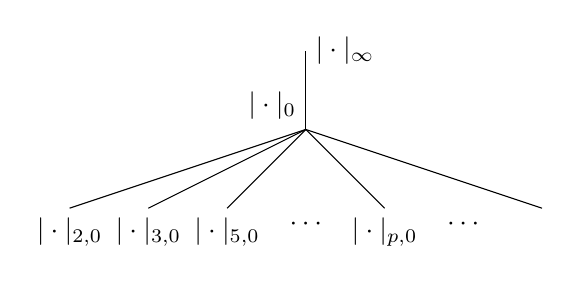
\begin{tikzpicture}%[scale = 0.5]
%	\draw[help lines] (0,0) grid (10,10);
	\draw (3,1) -- (3,2);
	\draw (0,0) -- (3,1);
	\draw (1,0) -- (3,1);
	\draw (2,0) -- (3,1);
	\draw (4,0) -- (3,1);
	\draw (6,0) -- (3,1);
	\node [right] at (3,2) {$|\cdot|_\infty$};
	\node [above left] at (3,1) {$|\cdot|_0$};
	\node [below] at (0,0) {$|\cdot|_{2,0}$};
	\node [below] at (1,0) {$|\cdot|_{3,0}$};
	\node [below] at (2,0) {$|\cdot|_{5,0}$};
	\node [below] at (3,0) {$\cdots$};
	\node [below] at (4,0) {$|\cdot|_{p,0}$};
	\node [below] at (5,0) {$\cdots$};
\end{tikzpicture}
\end{center}
\caption{The Berkovich spectrum $\Berkspec(\bZ)$}
\end{figure}

This picture is ``true,'' but you need 
to be careful: the Berkovich topology is \emph{not} the naive (metric) 
topology. Recall that $\Berkspec(\bZ)$ should carry the weakest topology 
making all maps $|\cdot|\mapsto |n|$ continuous. Since the norms in question 
are multiplicative, it suffices to ensure that the maps $|\cdot|\mapsto |p|$ 
are continuous for all primes $p$. In other words, the topology is generated by 
the sets 
\begin{align*}
	U_{p,t}^+ &= \{|\cdot|\colon |p|>t\} \\
	U_{p,t}^- &= \{|\cdot|\colon |p|<t\} .
\end{align*}
Define: 
\begin{align*}
	I_p &= \{|\cdot|_{p,\varepsilon}\colon 0\leqslant \varepsilon \leqslant 1\} \\
	I_\infty &= \{|\cdot|_{\infty,\varepsilon}\colon 0\leqslant \varepsilon \leqslant 1\} .
\end{align*}

\begin{proposition}
\leavevmode
\begin{enumerate}
\item
Any open set of $\Berkspec(\bZ)$ containing $|\cdot|_0$ contains all but 
finitely many $I_v$ for $v\in \{\text{primes}\}\cup\{\infty\}$. 

\item
The maps $[0,1]\to \Berkspec(\bZ)$, $\varepsilon\mapsto |\cdot|_{v,\varepsilon}$ 
are homeomorphisms onto the $I_v$. 
\end{enumerate}
\end{proposition}
\begin{proof}
1. Consider $U_{p,\varepsilon}^+$ for $t<1$. Recall that if $q\ne p$ is a prime, 
then $|q|_{p,\varepsilon}=1$. So $U_{p,t}^+\supset \bigcup_{v\ne p} I_v$. The 
similar statement holds for $U_{p,t}^-$. This (roughly) implies the first 
claim. 

2. It suffices to show that the maps $f_v\colon [0,1]\to I_v$ are continuous, as 
bijectivity is easy. Let $U_{q,\varepsilon}^+(p)=U_{q,\varepsilon}^+\cap I_p$. 
Then 
\[
  U_{q,\varepsilon}^+(p) = \begin{cases} I_p & t<1\text{ and }q\ne p \\ \varnothing & t>1\text{ and }q\ne p \\ \{|\cdot|_{p,\varepsilon}\colon \varepsilon>t\} & q=p \end{cases}
\]
So $f_p^{-1}(U_{q,\varepsilon}^+(p))$ will be either $[0,1]$, $\varnothing$, or 
$\{\varepsilon>t\}$. Similarly one handles $U_{q,\varepsilon}^-(p)$, and the 
infinite places. 
\end{proof}

Recall the ``kernel map'' $\ker\colon \Berkspec(\bZ)\to \spec(\bZ)$. It sends 
everything to the generic point $(0)$ \emph{except} the $|\cdot|_{p,0}$, which 
map to $(p)\in \spec(\bZ)$. 

The whole picture generalizes to rings of integers in number fields. 

Let $A$ be a Dedekind domain (integrally closed domain of dimension one) and 
$|\cdot|_0$ the trivial norm on $A$. Recall that the map 
$\ker\colon \Berkspec(A)\to \spec(A)$, $|\cdot|\mapsto \ker(|\cdot|)$, is 
continuous. We saw that there is a canonical section 
$\sigma\colon \spec(A)\to \Berkspec(A)$, which sends $\fp$ to the pullback of 
the trivial norm on $A/\fp$. However, $\sigma$ is not continuous, because 
$\Berkspec(A)$ is Hausdorff and $\spec(A)$ is not. 





\subsection{Reduction / specialization map}

Let $(A,|\cdot|)$ be a commutative Banach algebra, where $|\cdot|$ is 
non-archimedean. Define 
\begin{align*}
	A^\circ &= \{f\in A\colon \rho(f)\leqslant 1\} \\
	A^{\circ\circ} &= \{f\in A\colon \rho(f)<1\} .
\end{align*}
By \autoref{thm:rho}, $A^\circ$ is a ring and $A^{\circ\circ}$ is an ideal in 
$A^\circ$. So $A^\natural=A^\circ/A^{\circ\circ}$ is a ring (not necessarily a 
field, as $A^{\circ\circ}$ may not be maximal). We will define a \emph{reduction 
map} $\Berkspec(A)\to \spec(A^\natural)$. 

\begin{lemma}
Let $\varphi\colon A\to B$ be a bounded homomorphism of Banach rings. Then 
$\varphi$ induces maps 
\begin{align*}
	\varphi^\circ &\colon A^\circ\to B^\circ \\
	\varphi^{\circ\circ} &\colon A^{\circ\circ}\to B^{\circ\circ} \\ 
	\varphi^\natural &\colon A^\natural \to B^\natural .
\end{align*}
\end{lemma}
\begin{proof}
Clearly, it suffices to prove the first two parts. Better, it suffices to 
show that $\rho(\varphi(f))\leqslant \rho(f)$ for all $f\in A$. We know that 
there exists $C>0$ such that $\|\varphi(f)\|_B\leqslant C \|f\|_A$. The rest 
is an easy computation:
\begin{align*}
	\rho(\varphi(f)) 
		&= \lim_{n\to \infty} \|\varphi(f)^n\|^{1/n} \\
		&= \lim_{n\to \infty} \| \varphi(f^n)\|_B^{1/n} \\
		&\leqslant \lim_{n\to \infty} \left(C \|f^n\|_A\right)^{1/n} \\
		&= \lim_{n\to \infty} \|f^n\|^{1/n}_A = \rho(f) .
\end{align*}
\end{proof}

Let $x\in \Berkspec(A)$. We have an associated bounded homomorphism 
$\chi_x\colon A\to \sH(x)$. By the lemma, we get a homomorphism 
$\chi_x^\natural\colon A^\natural\to \sH(x)^\natural$. The field 
$\sH(x)^\natural$ is often written $\widetilde{\sH(x)}$ and called the 
\emph{double residue field} of $\Berkspec(A)$ at $x$. The ideal 
$\ker(\chi_x^\natural)\subset A^\natural$ is prime, so we have defined a map 
\[
	\red\colon \Berkspec(A)\to \spec(A^\natural) .
\]
If $\|\cdot\|=|\cdot|_0$ is the trivial norm on $A$, then 
\[
	\rho(f) = \begin{cases} 1 & f\text{ is not nilpotent} \\ 0 & f\text{ is nilpotent} \end{cases} 
\]
So $\ker(\rho)$ is the nilradical of $A$. Thus $A^\circ=A$, 
$A^{\circ\circ}=\rad(0)$, and $A^\natural=A/\rad(0)$. In particular, if $A$ is 
reduced, then $A^\natural=A$. 

For the moment, assume $A$ is reduced, and let $\|\cdot\|_A=|\cdot|_0$. We have 
a \emph{reduction map} $\red\colon \Berkspec(A)\to \spec(A)$, but this is 
\emph{not} the same as the ``kernel map'' 
$\ker\colon \Berkspec(A)\to \spec(A)$. Indeed, 
\[
	\red(x) = \{f\in A\colon |f(x)|<1\} \supset \{f\in A\colon |f(x)|=0\} = \ker(x) .
\]

If $K$ is a non-archimedean field and $A$ is a Banach $K$-algebra, then 
$A^\natural$ is a $K^\natural$-algebra. So $\spec(A^\natural)$ is a scheme over 
the residue field $K^\natural$. For example, if $K=\bQ_p$, then 
$K^\natural=\bF_p$ and the reduction map 
$\Berkspec(A)\to \spec(A^\natural)_{/\bF_p}$ takes values in a scheme over a 
finite field. This is why we call the map \emph{reduction} or 
\emph{specialization}. If $x\in \Berkspec(A)$, we have a point 
$x^\natural=\red(x)=\fp_{x^\natural}\in \spec(A^\natural)$. The algebraic 
residue field $k(x^\natural)$, namely $(A^\natural/\fp_{x^\natural})_{(0)}$, is 
canonically a subfield of $\sH(x)^\natural$. 

\begin{theorem}
Let $A$ be a noetherian Banach ring. Then the reduction map 
$\red\colon \Berkspec(A)\to \spec(A^\natural)$ is anticontinuous.
\end{theorem}
\begin{proof}
Recall that a map $f\colon X\to Y$ of topological spaces is 
\emph{anticontinuous} if $f^{-1}(\text{open})=\text{closed}$ and 
$f^{-1}(\text{closed})=\text{open}$. 

Let $\fa\subset A^\natural$ an ideal. Recall that the 
induced closed set $V(\fa)=\{\fp\in \spec(A^\natural)\colon \fa\in \fp\}$. Such 
closed sets define a topology on $\spec(A^\natural)$. It turns out that 
\[
	\red^{-1}(V(\fa)) = \{x\in \Berkspec(A)\colon |f(x)|<1\text{ for all }f+A^{\circ\circ}\in \fa\} .
\]
If $A$ is noetherian, the ideal $\fa+A^{\circ\circ}$ has a finite generating 
set $\langle f_1,\dots,f_n\rangle$, and 
\[
	\red^{-1}(V(\fa)) = \bigcap_i \{x\in \Berkspec(A)\colon |f_i(x)|<1\} .
\]
As a finite intersection of open sets, this is open. 
\end{proof}

If $A$ is a $K$-algebra, one could define the reduction map using the 
``valuative criterion of properness'' applied to $\spec(\sH(x))\to \fX$, 
where $\fX_{/K^\circ}$ is a proper flat model, assuming such a model exists. 





\subsection{Dedekind domains with trivial norm}

\begin{definition}
A commutative ring $A$ is called a \emph{Dedekind domain}  if it is an 
integrally closed, noetherian integral domain with Krull dimension $1$. 
\end{definition}

This definition is ``nice'' in the sense that it is usually easy to check if 
a given ring is Dedekind, but it is not immediately clear why we should care 
about Dedekind rings. 

\begin{theorem}
A noetherian integral domain $A$ is Dedekind if and only if any nonzero ideal 
$\fa\subset A$ factors uniquely as $\fa=\fp_1\cdots \fp_r$, where the $\fp_i$ 
are prime ideals. 
\end{theorem}

\begin{example}
If $F$ is a number field, then the ring of integers $O_F$ is Dedekind. For 
example, we could have $\bZ$, $\bZ[i]$, 
$\bZ\left[\frac{\sqrt{-3}+1}{2}\right]$, etc.
\end{example}

\begin{example}
A curve $C$ is nonsingular if and only if for all $U\subset C$ open, the 
ring $\h^0(U,\sO)$ is Dedekind. This is because one-dimensional varieties are 
normal if and only if they are smooth. 
\end{example}

So proper algebraic curves are a kind of ``geometrization'' of the notion of 
a Dedekind domain. 

\begin{lemma}
A noetherian domain $A$ is Dedekind if and only if $A_\fp$ is a discrete 
valuation ring for all nonzero primes $\fp\subset A$. 
\end{lemma}

Let $A$ be a Dedekind domain with trivial norm $|\cdot|_0$. We'd like to 
understand $\Berkspec(A)$. 
\begin{center}
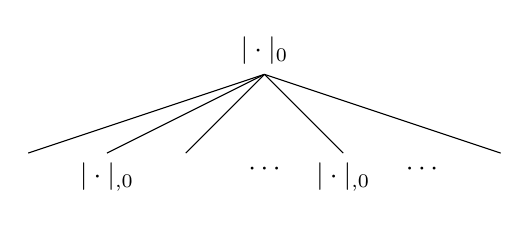
\begin{tikzpicture}
	\draw (0,0) -- (3,1);
	\draw (1,0) -- (3,1);
	\draw (2,0) -- (3,1);
	\draw (4,0) -- (3,1);
	\draw (6,0) -- (3,1);
	\node [above] at (3,1) {$|\cdot|_0$};
	\node [below] at (1,0) {$|\cdot|_{\fp,0}$};
	\node [below] at (3,0) {$\cdots$};
	\node [below] at (4,0) {$|\cdot|_{\fq,0}$};
	\node [below] at (5,0) {$\cdots$};
\end{tikzpicture}
\end{center}
Fix $x\in \Berkspec(A)$, and let $\fp_x=\ker(x)=\{f\in A\colon |f(x)|=0\}$. 
Let $\fq_x=\red(x) = \{f\in A\colon |f(x)|<1\}$. Clearly $\fp_x\subset \fq_x$. 
If $\fp_x\ne 0$, then $\dim(A)=1$ forces $\fp_x=\fq_x$. If $\fp_x=0$, there 
are two possibilities: either $\fq_x=0$ or $\fq_x\ne 0$. 

Case 1: $\fp_x\ne 0$. Then
\[
	|f| _x= \begin{cases} 0 & f\in \fp_x \\ 1 & f\notin \fp_x \end{cases}
\]
because $|f(x)| \leqslant |f|_0 = 1$ and $|f(x)|<1$ if and only if $|f(x)|=0$, 
if and only if $f\in \fp_x$. So $|\cdot|_x$ is the image of $\fp_x=\fp$ under 
the canonical section $\spec(A)\to \Berkspec(A)$. Call this norm 
$|\cdot|_{\fp,0}$. 

Case 2: $0=\fp_x= \fq_x$. One handles this exactly as in Case 1. We get that 
$|\cdot|_x=|\cdot|_0$. 

Case 3: $0=\fp_x\subsetneq \fq_x$. In the map $A\to A_{\fq_x}$, the target is 
a discrete valuation ring. The norm $|\cdot|_x$ extends to a multiplicative 
norm on $A_{\fq_x}$. Fix a generator $\pi$ for the maximal ideal 
$\fm=(\fq_x)_{\fq_x}$ of $A_{\fq_x}$. The natural valuation on $A_{\fq_x}$ is 
\[
	\valuation'(\varepsilon \pi^i) = i 
\]
whenever $\varepsilon\in A_{\fq_x}^\times$. If $\valuation_t$ is some other 
valuation with $\valuation(\pi)=t$, then $\valuation_t=t\valuation'$. So for 
$0<t<\infty$, we have a multiplicative seminorm on $A$, restricted from one on 
$A_{\fq_x}$, given by 
\[
	|\cdot|_{\fq,t^{-1}} = e^{-\valuation_t} .
\]
As $t\to 0^+$, $|\cdot|_{\fq,t^{-1}}\to |\cdot|_0$, and as $t\to \infty$, 
$|\cdot|_{\fq,t^{-1}} \to |\cdot|_{\fq,0}$. 





\subsection{Berkovich unit disk}

We consider convergent power series in one variable (i.e.~analytic functions). 
The spectrum of this algebra will be the ``Berkovich closed disk.''

Fix a field $K$ complete with respect to an absolute value $|\cdot|$. We do not 
assume $K$ is non-archimedean, so we could have $K=\bR$. Let $r>0$, and define 
\[
	A = K\respow{r^{-1} T} = \left\{\sum_{i\geqslant 0} a_i T^i\colon \|f\| = \sum |a_i| r^i < \infty \right\} .
\]
We want to think of $\Berkspec(A)$ as the closed analytic disk with radius $r$. 
The norm $\|\cdot\|$ is not even power-multiplicative (i.e., $A$ is not a 
uniform algebra), which makes certain computations very annoying. What is 
$A^\mathrm{u}$? In other words, what is the spectral radius norm $\rho(\cdot)$ 
on $A$, and the completion of $A$ with respect to $\rho$? Since 
$\Berkspec(A)=\Berkspec(A^\mathrm{u})$, we still have the same rigid-analytic 
space. 

\begin{theorem}
Let $f=\sum_{i\geqslant 0} a_i T^i\in K\respow{r^{-1} T}$. 
\begin{enumerate}
\item
If $K$ is non-archimedean, then 
\begin{align*}
	\rho(f) &= \max_{i\geqslant 0} |a_i| r^i \\
	A^\mathrm{u} &= K\conpow{r^{-1} T} = \left\{f=\sum a_i T^i\colon \lim_{i\to \infty} |a_i| r^i = 0\right\} .
\end{align*}

\item
If $K=\bC$, put $D_r=\{z\in \bC\colon |z|\leqslant r\}$, 
$D_r^-=\{z\in \bC\colon |z|<r\}$. 
\begin{align*}
	\rho(f) &= \max_{z\in D_r} |f(z)| \\
	A^\mathrm{u} &= \{f\in \sC(D,\bC)\colon f|_{D^-}\text{ is analytic}\} .
\end{align*}

\item
If $K=\bR$, then $\rho$ is the restriction of the above $\rho$ to real-analytic 
functions, and $A^\mathrm{u}$ is the subalgebra of $(A_\bC)^\mathrm{u}$ with 
real Taylor coefficients. 

\item
If $K$ is non-archimedean, then $\rho(\cdot)$ multiplicative. 
\end{enumerate}
\end{theorem}
\begin{proof}
We will ignore the archimedean case, as this essentially follows from the 
discussion on Gelfand's theory. So assume $K$ is non-archimedean.

1. Let $|f|=\max |a_i| r^i$. First we show $\rho(f) \geqslant |f|$. Clearly 
$|f|\leqslant \|f\|$. We show later that $|\cdot|$ is power-multiplicative. 
Assuming this, we have 
\[
  \rho(f) = \lim_{n\to \infty} \|f^n\|^{1/n} \geqslant \lim_{n\to \infty} |f^n|^{1/n} = |f| .
\]
Now we show $\rho(f) \leqslant |f|$. First, assume $f\in K\respow{r^{-1} T}$ is 
a polynomial. Then $|f| = \max |a_i|r^i \geqslant |a_j| r^j$ for all 
$j\geqslant 0$. In other words, $|a_j| \leqslant |f| r^{-j}$. We now compute: 
\[
	\|f\| = \sum_{j\leqslant \deg f} |a_j| r^j \leqslant \sum_{j\leqslant \deg f} |f| r^{-j} r^j = \sum_{j\leqslant \deg f} |f| = (1+\deg f)|f| .
\]
So in general, 
\[
	\|f^n\|^{1/n} \leqslant (1+n\deg f)^{1/n} |f^n|^{1/n} ,
\]
whence $\rho(f) \leqslant |f|$. Assume for now that $r=1$. By the 
Weierstrass Preparation Theorem, for any $f\in K\conpow{T}$, there exists a 
polynomial $g\in K[T]$ and $h\in K\conpow{T}$ of the form 
$h=1+\sum_{i>0} a_i T^i$ with $|b_i|<1$, such that $f = g h$. One checks 
that $|h|=1$, and that $\rho(h)\leqslant 1$, using the definition of $\rho$. 
So 
\[
	\rho(f) = \rho(g h) \leqslant \rho(g) \rho(h) \leqslant |g|\cdot 1 = |g h| = |f| . 
\]
Alternatively, polynomials are dense in $(K\respow{r^{-1}T},\|\cdot\|)$. So 
for $f\in K\respow{r^{-1} T}$, there exists $\{p_n\}\subset K[T]$ such that 
$p_n\to f$. If $|f|<\rho(f)$, then since $|p_n|\geqslant \rho(p_n)$ for all 
$n$, we get a contradiction. 

4. That $|f g| \leqslant |f| |g|$ is clear from the definition. To show 
equality, we first assume $r=1$. Then 
$A^\circ = \{f\colon |f|\leqslant 1\} = K^\circ\pow{T}$, and 
$A^{\circ\circ} = K^{\circ\circ}\pow{T}$. The ``residue ring'' 
$A^\natural = K^\natural[T]$, which is not a field.  Write 
$\pi\colon A\to A^\natural$ for the projection. Note that 
$\pi(f)\ne 0$ if and only if $|f|=1$. Assume $|f|=|g|=1$. Then 
$\pi(f),\pi(g)\ne 0$, so $\pi(f g)\ne 0$, hence $|f g|=1$. 
\end{proof}

By part 4, the spectral norm $\rho(\cdot)\in \Berkspec(A^\mathrm{u})$. One 
calls $\rho$ the \emph{Gauss norm} because the proof of its multiplicativity 
uses Gauss' lemma about the factorization of polynomials. In rigid-analytic 
geometry, $(K\conpow{T},\rho)$ is called the \emph{Tate algebra} in one 
variable. Since $\rho$ is multiplicative, $K\conpow{r^{-1} T}$ is an 
integral domain. 
